\documentclass[]{article}
\usepackage{lmodern}
\usepackage{amssymb,amsmath}
\usepackage{ifxetex,ifluatex}
\usepackage{fixltx2e} % provides \textsubscript
\ifnum 0\ifxetex 1\fi\ifluatex 1\fi=0 % if pdftex
  \usepackage[T1]{fontenc}
  \usepackage[utf8]{inputenc}
\else % if luatex or xelatex
  \ifxetex
    \usepackage{mathspec}
  \else
    \usepackage{fontspec}
  \fi
  \defaultfontfeatures{Ligatures=TeX,Scale=MatchLowercase}
\fi
% use upquote if available, for straight quotes in verbatim environments
\IfFileExists{upquote.sty}{\usepackage{upquote}}{}
% use microtype if available
\IfFileExists{microtype.sty}{%
\usepackage{microtype}
\UseMicrotypeSet[protrusion]{basicmath} % disable protrusion for tt fonts
}{}
\usepackage[margin=1in]{geometry}
\usepackage{hyperref}
\hypersetup{unicode=true,
            pdftitle={Bude},
            pdfauthor={Brianna Kincaid},
            pdfborder={0 0 0},
            breaklinks=true}
\urlstyle{same}  % don't use monospace font for urls
\usepackage{color}
\usepackage{fancyvrb}
\newcommand{\VerbBar}{|}
\newcommand{\VERB}{\Verb[commandchars=\\\{\}]}
\DefineVerbatimEnvironment{Highlighting}{Verbatim}{commandchars=\\\{\}}
% Add ',fontsize=\small' for more characters per line
\usepackage{framed}
\definecolor{shadecolor}{RGB}{248,248,248}
\newenvironment{Shaded}{\begin{snugshade}}{\end{snugshade}}
\newcommand{\AlertTok}[1]{\textcolor[rgb]{0.94,0.16,0.16}{#1}}
\newcommand{\AnnotationTok}[1]{\textcolor[rgb]{0.56,0.35,0.01}{\textbf{\textit{#1}}}}
\newcommand{\AttributeTok}[1]{\textcolor[rgb]{0.77,0.63,0.00}{#1}}
\newcommand{\BaseNTok}[1]{\textcolor[rgb]{0.00,0.00,0.81}{#1}}
\newcommand{\BuiltInTok}[1]{#1}
\newcommand{\CharTok}[1]{\textcolor[rgb]{0.31,0.60,0.02}{#1}}
\newcommand{\CommentTok}[1]{\textcolor[rgb]{0.56,0.35,0.01}{\textit{#1}}}
\newcommand{\CommentVarTok}[1]{\textcolor[rgb]{0.56,0.35,0.01}{\textbf{\textit{#1}}}}
\newcommand{\ConstantTok}[1]{\textcolor[rgb]{0.00,0.00,0.00}{#1}}
\newcommand{\ControlFlowTok}[1]{\textcolor[rgb]{0.13,0.29,0.53}{\textbf{#1}}}
\newcommand{\DataTypeTok}[1]{\textcolor[rgb]{0.13,0.29,0.53}{#1}}
\newcommand{\DecValTok}[1]{\textcolor[rgb]{0.00,0.00,0.81}{#1}}
\newcommand{\DocumentationTok}[1]{\textcolor[rgb]{0.56,0.35,0.01}{\textbf{\textit{#1}}}}
\newcommand{\ErrorTok}[1]{\textcolor[rgb]{0.64,0.00,0.00}{\textbf{#1}}}
\newcommand{\ExtensionTok}[1]{#1}
\newcommand{\FloatTok}[1]{\textcolor[rgb]{0.00,0.00,0.81}{#1}}
\newcommand{\FunctionTok}[1]{\textcolor[rgb]{0.00,0.00,0.00}{#1}}
\newcommand{\ImportTok}[1]{#1}
\newcommand{\InformationTok}[1]{\textcolor[rgb]{0.56,0.35,0.01}{\textbf{\textit{#1}}}}
\newcommand{\KeywordTok}[1]{\textcolor[rgb]{0.13,0.29,0.53}{\textbf{#1}}}
\newcommand{\NormalTok}[1]{#1}
\newcommand{\OperatorTok}[1]{\textcolor[rgb]{0.81,0.36,0.00}{\textbf{#1}}}
\newcommand{\OtherTok}[1]{\textcolor[rgb]{0.56,0.35,0.01}{#1}}
\newcommand{\PreprocessorTok}[1]{\textcolor[rgb]{0.56,0.35,0.01}{\textit{#1}}}
\newcommand{\RegionMarkerTok}[1]{#1}
\newcommand{\SpecialCharTok}[1]{\textcolor[rgb]{0.00,0.00,0.00}{#1}}
\newcommand{\SpecialStringTok}[1]{\textcolor[rgb]{0.31,0.60,0.02}{#1}}
\newcommand{\StringTok}[1]{\textcolor[rgb]{0.31,0.60,0.02}{#1}}
\newcommand{\VariableTok}[1]{\textcolor[rgb]{0.00,0.00,0.00}{#1}}
\newcommand{\VerbatimStringTok}[1]{\textcolor[rgb]{0.31,0.60,0.02}{#1}}
\newcommand{\WarningTok}[1]{\textcolor[rgb]{0.56,0.35,0.01}{\textbf{\textit{#1}}}}
\usepackage{graphicx,grffile}
\makeatletter
\def\maxwidth{\ifdim\Gin@nat@width>\linewidth\linewidth\else\Gin@nat@width\fi}
\def\maxheight{\ifdim\Gin@nat@height>\textheight\textheight\else\Gin@nat@height\fi}
\makeatother
% Scale images if necessary, so that they will not overflow the page
% margins by default, and it is still possible to overwrite the defaults
% using explicit options in \includegraphics[width, height, ...]{}
\setkeys{Gin}{width=\maxwidth,height=\maxheight,keepaspectratio}
\IfFileExists{parskip.sty}{%
\usepackage{parskip}
}{% else
\setlength{\parindent}{0pt}
\setlength{\parskip}{6pt plus 2pt minus 1pt}
}
\setlength{\emergencystretch}{3em}  % prevent overfull lines
\providecommand{\tightlist}{%
  \setlength{\itemsep}{0pt}\setlength{\parskip}{0pt}}
\setcounter{secnumdepth}{0}
% Redefines (sub)paragraphs to behave more like sections
\ifx\paragraph\undefined\else
\let\oldparagraph\paragraph
\renewcommand{\paragraph}[1]{\oldparagraph{#1}\mbox{}}
\fi
\ifx\subparagraph\undefined\else
\let\oldsubparagraph\subparagraph
\renewcommand{\subparagraph}[1]{\oldsubparagraph{#1}\mbox{}}
\fi

%%% Use protect on footnotes to avoid problems with footnotes in titles
\let\rmarkdownfootnote\footnote%
\def\footnote{\protect\rmarkdownfootnote}

%%% Change title format to be more compact
\usepackage{titling}

% Create subtitle command for use in maketitle
\newcommand{\subtitle}[1]{
  \posttitle{
    \begin{center}\large#1\end{center}
    }
}

\setlength{\droptitle}{-2em}
  \title{Bude}
  \pretitle{\vspace{\droptitle}\centering\huge}
  \posttitle{\par}
  \author{Brianna Kincaid}
  \preauthor{\centering\large\emph}
  \postauthor{\par}
  \predate{\centering\large\emph}
  \postdate{\par}
  \date{March 21, 2018}


\begin{document}
\maketitle

\hypertarget{set-up}{%
\section{Set up}\label{set-up}}

First import necessary libraries.

\begin{Shaded}
\begin{Highlighting}[]
\KeywordTok{library}\NormalTok{(ggmap)}
\end{Highlighting}
\end{Shaded}

\begin{verbatim}
## Loading required package: ggplot2
\end{verbatim}

\begin{Shaded}
\begin{Highlighting}[]
\KeywordTok{library}\NormalTok{(tidyverse)}
\end{Highlighting}
\end{Shaded}

\begin{verbatim}
## -- Attaching packages ---------------------------------------------------------------------------------------------- tidyverse 1.2.1 --
\end{verbatim}

\begin{verbatim}
## √ tibble  1.4.2     √ purrr   0.2.4
## √ tidyr   0.8.0     √ dplyr   0.7.4
## √ readr   1.1.1     √ stringr 1.3.0
## √ tibble  1.4.2     √ forcats 0.3.0
\end{verbatim}

\begin{verbatim}
## -- Conflicts ------------------------------------------------------------------------------------------------- tidyverse_conflicts() --
## x dplyr::filter() masks stats::filter()
## x dplyr::lag()    masks stats::lag()
\end{verbatim}

\begin{Shaded}
\begin{Highlighting}[]
\KeywordTok{library}\NormalTok{(knitr)}
\end{Highlighting}
\end{Shaded}

Bude is a town in Western England, well-known as a beach resort. We find
the coordinates using \texttt{geocode()}.

\begin{Shaded}
\begin{Highlighting}[]
\NormalTok{Bude_coord <-}\StringTok{ }\KeywordTok{geocode}\NormalTok{(}\StringTok{"S W Coast Path, Bude EX23 8HN, UK"}\NormalTok{) }
\end{Highlighting}
\end{Shaded}

\begin{verbatim}
## Information from URL : http://maps.googleapis.com/maps/api/geocode/json?address=S%20W%20Coast%20Path,%20Bude%20EX23%208HN,%20UK&sensor=false
\end{verbatim}

I chose the center of the map to be the Bude North Cornwall Cricket
Club, as that is the central location of this assignment, and allows for
better viewing of the surrounding area.

\hypertarget{road-map}{%
\section{Road map}\label{road-map}}

\begin{Shaded}
\begin{Highlighting}[]
\NormalTok{Bude_roadmap <-}\StringTok{ }\KeywordTok{get_map}\NormalTok{(Bude_coord, }\DataTypeTok{zoom =} \DecValTok{15}\NormalTok{)}
\end{Highlighting}
\end{Shaded}

\begin{verbatim}
## Map from URL : http://maps.googleapis.com/maps/api/staticmap?center=50.832584,-4.553165&zoom=15&size=640x640&scale=2&maptype=terrain&language=en-EN&sensor=false
\end{verbatim}

\begin{Shaded}
\begin{Highlighting}[]
\KeywordTok{ggmap}\NormalTok{(Bude_roadmap)}
\end{Highlighting}
\end{Shaded}

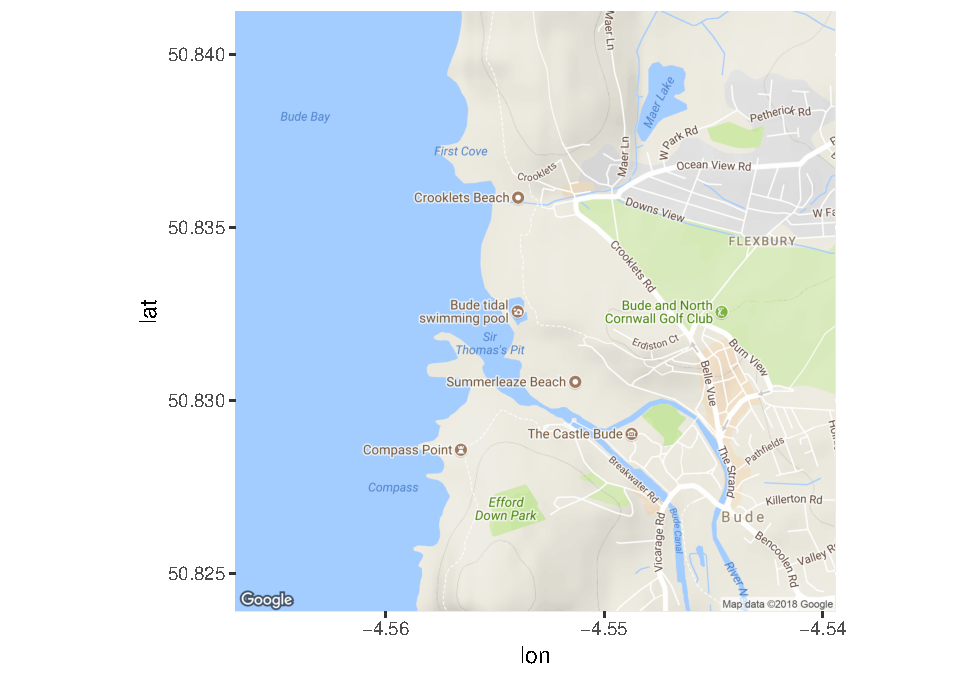
\includegraphics{Bude_files/figure-latex/unnamed-chunk-4-1.pdf}

\hypertarget{watercolor-map}{%
\section{Watercolor map}\label{watercolor-map}}

\begin{Shaded}
\begin{Highlighting}[]
\NormalTok{Bude_watercolor <-}\StringTok{ }\KeywordTok{get_map}\NormalTok{(Bude_coord, }\DataTypeTok{maptype =} \StringTok{"watercolor"}\NormalTok{, }\DataTypeTok{zoom =} \DecValTok{15}\NormalTok{)}
\end{Highlighting}
\end{Shaded}

\begin{verbatim}
## maptype = "watercolor" is only available with source = "stamen".
\end{verbatim}

\begin{verbatim}
## resetting to source = "stamen"...
\end{verbatim}

\begin{verbatim}
## Map from URL : http://maps.googleapis.com/maps/api/staticmap?center=50.832584,-4.553165&zoom=15&size=640x640&scale=2&maptype=terrain&sensor=false
\end{verbatim}

\begin{verbatim}
## Map from URL : http://tile.stamen.com/watercolor/15/15968/10992.jpg
\end{verbatim}

\begin{verbatim}
## Map from URL : http://tile.stamen.com/watercolor/15/15969/10992.jpg
\end{verbatim}

\begin{verbatim}
## Map from URL : http://tile.stamen.com/watercolor/15/15970/10992.jpg
\end{verbatim}

\begin{verbatim}
## Map from URL : http://tile.stamen.com/watercolor/15/15968/10993.jpg
\end{verbatim}

\begin{verbatim}
## Map from URL : http://tile.stamen.com/watercolor/15/15969/10993.jpg
\end{verbatim}

\begin{verbatim}
## Map from URL : http://tile.stamen.com/watercolor/15/15970/10993.jpg
\end{verbatim}

\begin{verbatim}
## Map from URL : http://tile.stamen.com/watercolor/15/15968/10994.jpg
\end{verbatim}

\begin{verbatim}
## Map from URL : http://tile.stamen.com/watercolor/15/15969/10994.jpg
\end{verbatim}

\begin{verbatim}
## Map from URL : http://tile.stamen.com/watercolor/15/15970/10994.jpg
\end{verbatim}

\begin{verbatim}
## Map from URL : http://tile.stamen.com/watercolor/15/15968/10995.jpg
\end{verbatim}

\begin{verbatim}
## Map from URL : http://tile.stamen.com/watercolor/15/15969/10995.jpg
\end{verbatim}

\begin{verbatim}
## Map from URL : http://tile.stamen.com/watercolor/15/15970/10995.jpg
\end{verbatim}

\begin{Shaded}
\begin{Highlighting}[]
\KeywordTok{ggmap}\NormalTok{(Bude_watercolor)}
\end{Highlighting}
\end{Shaded}

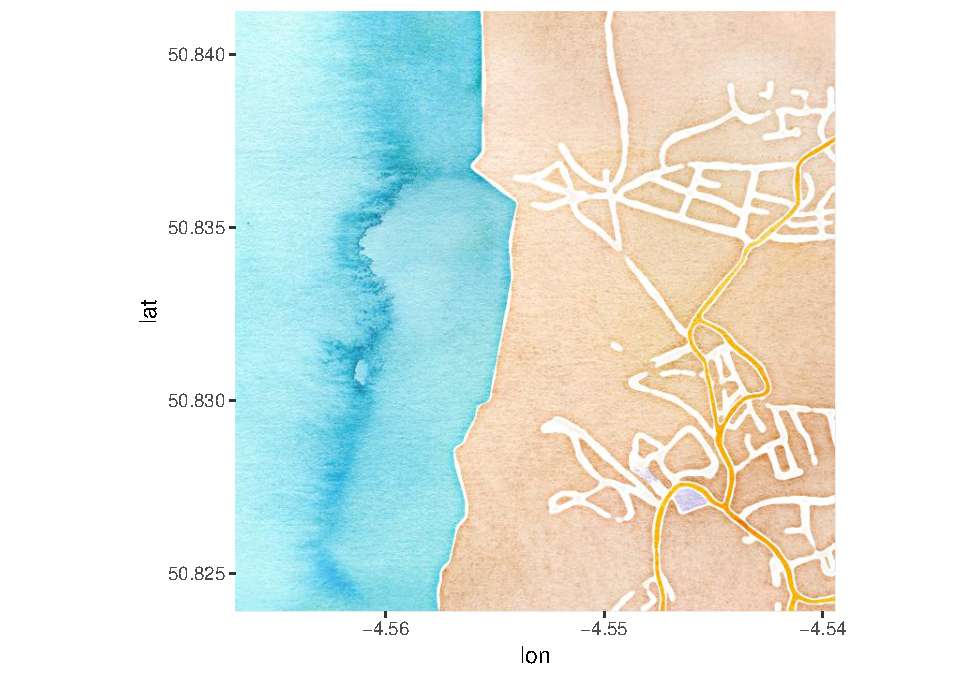
\includegraphics{Bude_files/figure-latex/unnamed-chunk-6-1.pdf}

\hypertarget{marking-vacation-spots}{%
\section{Marking vacation spots}\label{marking-vacation-spots}}

There are a number of good beaches in the Bude area, many of which offer
good surfing conditions.

\hypertarget{two-local-beaches}{%
\subsection{Two local beaches}\label{two-local-beaches}}

\hypertarget{summerleaze-beach}{%
\subsubsection{Summerleaze Beach}\label{summerleaze-beach}}

\begin{Shaded}
\begin{Highlighting}[]
\KeywordTok{include_graphics}\NormalTok{(}\StringTok{"summerleaze.jpg"}\NormalTok{)}
\end{Highlighting}
\end{Shaded}

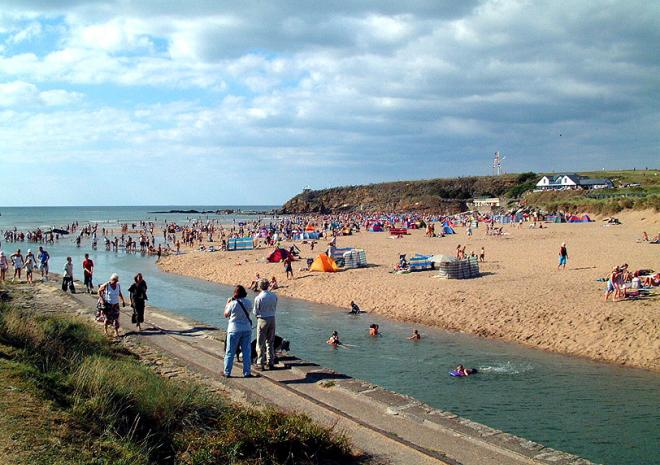
\includegraphics[width=0.5\linewidth]{summerleaze}

\begin{Shaded}
\begin{Highlighting}[]
\NormalTok{summerleaze <-}\StringTok{ }\KeywordTok{geocode}\NormalTok{(}\StringTok{"Summerleaze Beach, Summerleaze Cres, Bude EX23 8HN, UK"}\NormalTok{)}
\end{Highlighting}
\end{Shaded}

\begin{verbatim}
## Information from URL : http://maps.googleapis.com/maps/api/geocode/json?address=Summerleaze%20Beach,%20Summerleaze%20Cres,%20Bude%20EX23%208HN,%20UK&sensor=false
\end{verbatim}

\hypertarget{crooklets-beach}{%
\subsubsection{Crooklets Beach}\label{crooklets-beach}}

\begin{Shaded}
\begin{Highlighting}[]
\KeywordTok{include_graphics}\NormalTok{(}\StringTok{"crooklets.jpg"}\NormalTok{)}
\end{Highlighting}
\end{Shaded}

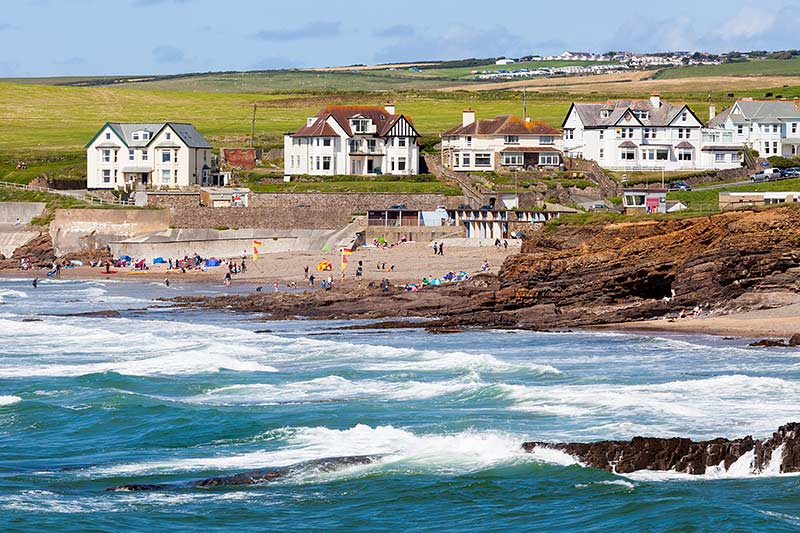
\includegraphics[width=2\linewidth]{crooklets}

\begin{Shaded}
\begin{Highlighting}[]
\NormalTok{crooklets <-}\StringTok{ }\KeywordTok{geocode}\NormalTok{(}\StringTok{"Crooklets Beach, S W Coast Path, Bude EX23 8NE, UK"}\NormalTok{)}
\end{Highlighting}
\end{Shaded}

\begin{verbatim}
## Information from URL : http://maps.googleapis.com/maps/api/geocode/json?address=Crooklets%20Beach,%20S%20W%20Coast%20Path,%20Bude%20EX23%208NE,%20UK&sensor=false
\end{verbatim}

\hypertarget{cricket-grounds-bude-north-cornwall-cricket-club}{%
\subsubsection{Cricket grounds (Bude North Cornwall Cricket
Club)}\label{cricket-grounds-bude-north-cornwall-cricket-club}}

``Bude North Cornwall Cricket Club is situated on the clifftops
overlooking the Atlantic Ocean, and is quite simply one of the most
stunning locations you could ever wish to visit, let alone play cricket
at! Bude North Cornwall Cricket Club was founded in 1870. Over the years
it has played host to Hockey matches, Tennis, Cricket and even used for
Mortar practice in WW2!''
\href{http://budecc.play-cricket.com/}{Source.}

\begin{Shaded}
\begin{Highlighting}[]
\KeywordTok{include_graphics}\NormalTok{(}\StringTok{"cricket.jpg"}\NormalTok{)}
\end{Highlighting}
\end{Shaded}

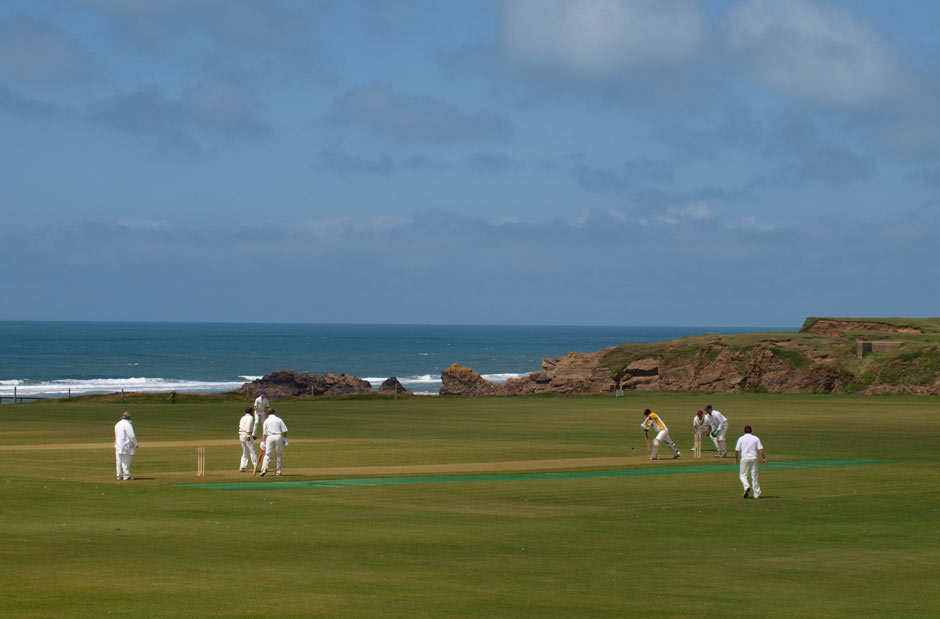
\includegraphics[width=0.25\linewidth]{cricket}

\begin{Shaded}
\begin{Highlighting}[]
\NormalTok{cricket_grounds_coord <-}\KeywordTok{geocode}\NormalTok{(}\StringTok{"Bude North Cornwall Cricket Club"}\NormalTok{)}
\end{Highlighting}
\end{Shaded}

\begin{verbatim}
## Information from URL : http://maps.googleapis.com/maps/api/geocode/json?address=Bude%20North%20Cornwall%20Cricket%20Club&sensor=false
\end{verbatim}

\hypertarget{oak-lodge-bed-and-breakfast}{%
\subsubsection{Oak Lodge Bed and
Breakfast}\label{oak-lodge-bed-and-breakfast}}

\begin{Shaded}
\begin{Highlighting}[]
\KeywordTok{include_graphics}\NormalTok{(}\StringTok{"oaklodge.jpg"}\NormalTok{)}
\end{Highlighting}
\end{Shaded}

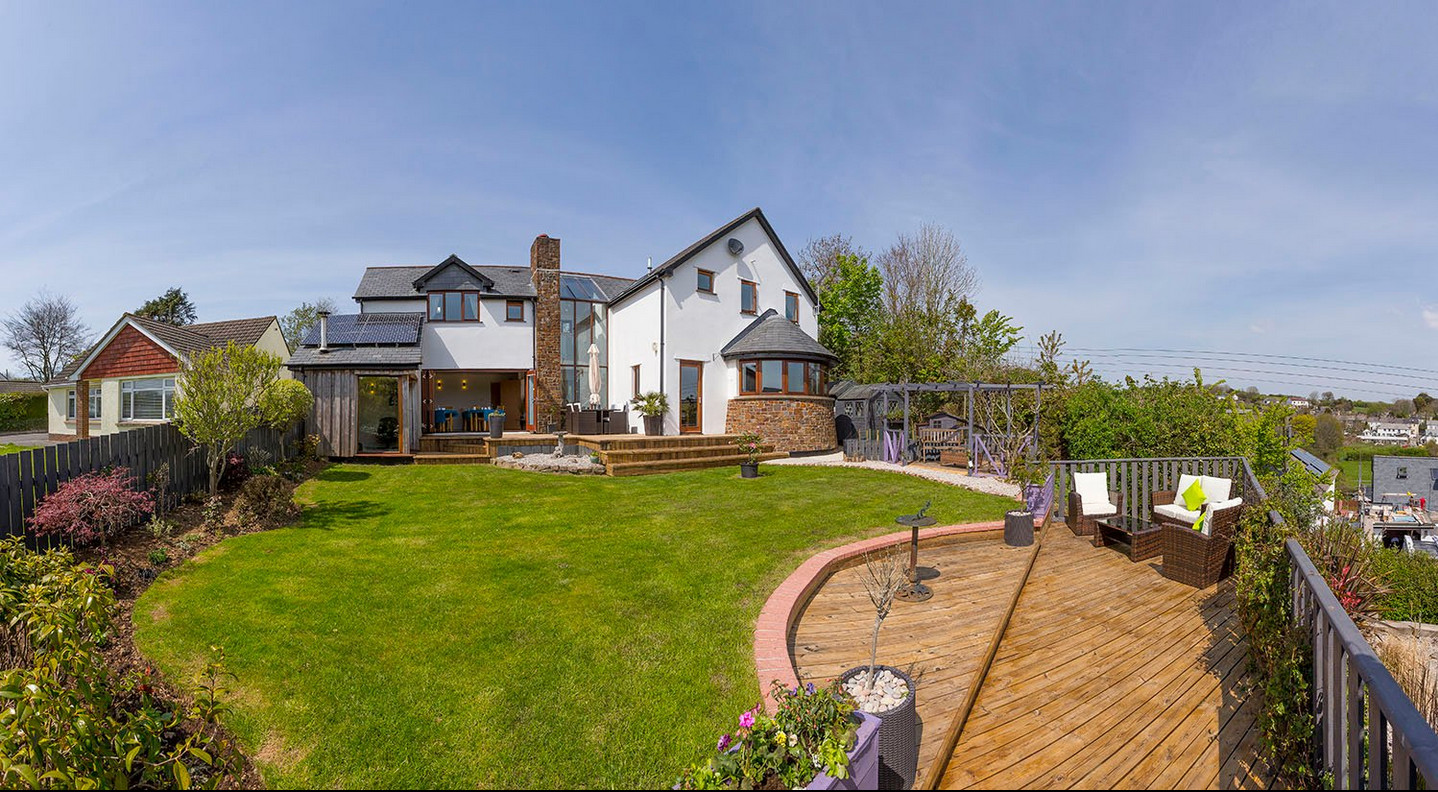
\includegraphics[width=0.25\linewidth]{oaklodge}

\begin{Shaded}
\begin{Highlighting}[]
\NormalTok{lodge_coord <-}\KeywordTok{geocode}\NormalTok{(}\StringTok{"Stratton, Bude EX23 9AT, England"}\NormalTok{)}
\end{Highlighting}
\end{Shaded}

\begin{verbatim}
## Information from URL : http://maps.googleapis.com/maps/api/geocode/json?address=Stratton,%20Bude%20EX23%209AT,%20England&sensor=false
\end{verbatim}

\hypertarget{falcon-hotel}{%
\subsubsection{Falcon Hotel}\label{falcon-hotel}}

\begin{Shaded}
\begin{Highlighting}[]
\KeywordTok{include_graphics}\NormalTok{(}\StringTok{"hotel.jpg"}\NormalTok{)}
\end{Highlighting}
\end{Shaded}

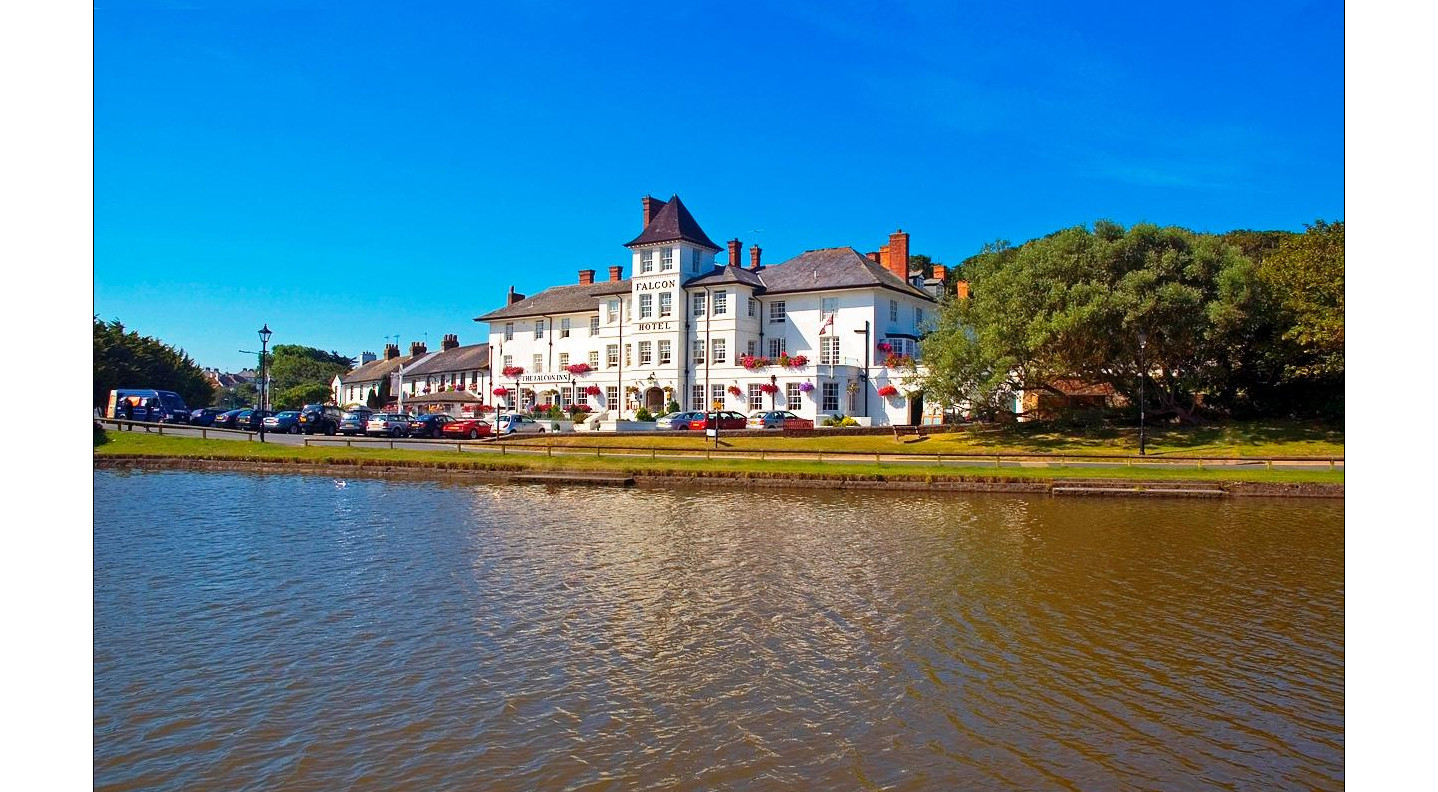
\includegraphics[width=0.25\linewidth]{hotel}

\begin{Shaded}
\begin{Highlighting}[]
\NormalTok{hotel_coord <-}\KeywordTok{geocode}\NormalTok{(}\StringTok{"Breakwater Road, Bude EX23 8SD, England"}\NormalTok{)}
\end{Highlighting}
\end{Shaded}

\begin{verbatim}
## Information from URL : http://maps.googleapis.com/maps/api/geocode/json?address=Breakwater%20Road,%20Bude%20EX23%208SD,%20England&sensor=false
\end{verbatim}

\hypertarget{putting-them-on-the-maps}{%
\subsubsection{Putting them on the
maps}\label{putting-them-on-the-maps}}

\begin{Shaded}
\begin{Highlighting}[]
\KeywordTok{ggmap}\NormalTok{(Bude_roadmap) }\OperatorTok{+}
\StringTok{  }\KeywordTok{geom_point}\NormalTok{(}\DataTypeTok{mapping =} \KeywordTok{aes}\NormalTok{(}\DataTypeTok{x =}\NormalTok{ summerleaze}\OperatorTok{$}\NormalTok{lon, }\DataTypeTok{y =}\NormalTok{ summerleaze}\OperatorTok{$}\NormalTok{lat)) }\OperatorTok{+}
\StringTok{  }\KeywordTok{geom_label}\NormalTok{(}\DataTypeTok{x =}\NormalTok{ summerleaze}\OperatorTok{$}\NormalTok{lon, }\DataTypeTok{y =}\NormalTok{ summerleaze}\OperatorTok{$}\NormalTok{lat, }\DataTypeTok{label =} \StringTok{"Summerleaze Beach"}\NormalTok{, }\DataTypeTok{hjust =} \DecValTok{1}\NormalTok{, }\DataTypeTok{vjust=}\DecValTok{1}\NormalTok{) }\OperatorTok{+}
\StringTok{  }\KeywordTok{geom_point}\NormalTok{(}\DataTypeTok{mapping =} \KeywordTok{aes}\NormalTok{(}\DataTypeTok{x =}\NormalTok{ crooklets}\OperatorTok{$}\NormalTok{lon, }\DataTypeTok{y =}\NormalTok{ crooklets}\OperatorTok{$}\NormalTok{lat)) }\OperatorTok{+}
\StringTok{  }\KeywordTok{geom_label}\NormalTok{(}\DataTypeTok{x =}\NormalTok{ crooklets}\OperatorTok{$}\NormalTok{lon, }\DataTypeTok{y =}\NormalTok{ crooklets}\OperatorTok{$}\NormalTok{lat, }\DataTypeTok{label =} \StringTok{"Crooklets Beach"}\NormalTok{, }\DataTypeTok{hjust =} \DecValTok{1}\NormalTok{, }\DataTypeTok{vjust=}\DecValTok{1}\NormalTok{) }\OperatorTok{+}
\StringTok{  }\KeywordTok{geom_point}\NormalTok{(}\DataTypeTok{mapping =} \KeywordTok{aes}\NormalTok{(}\DataTypeTok{x =}\NormalTok{ cricket_grounds_coord}\OperatorTok{$}\NormalTok{lon, }\DataTypeTok{y =}\NormalTok{ cricket_grounds_coord}\OperatorTok{$}\NormalTok{lat)) }\OperatorTok{+}
\StringTok{  }\KeywordTok{geom_label}\NormalTok{(}\DataTypeTok{x =}\NormalTok{ cricket_grounds_coord}\OperatorTok{$}\NormalTok{lon, }\DataTypeTok{y =}\NormalTok{ cricket_grounds_coord}\OperatorTok{$}\NormalTok{lat, }\DataTypeTok{label =} \StringTok{"Cricket Grounds"}\NormalTok{, }\DataTypeTok{hjust =} \DecValTok{1}\NormalTok{, }\DataTypeTok{vjust =} \DecValTok{1}\NormalTok{) }\OperatorTok{+}
\StringTok{  }\KeywordTok{geom_point}\NormalTok{(}\DataTypeTok{mapping =} \KeywordTok{aes}\NormalTok{(}\DataTypeTok{x =}\NormalTok{ lodge_coord}\OperatorTok{$}\NormalTok{lon, }\DataTypeTok{y =}\NormalTok{ lodge_coord}\OperatorTok{$}\NormalTok{lat)) }\OperatorTok{+}
\StringTok{  }\KeywordTok{geom_label}\NormalTok{(}\DataTypeTok{x =}\NormalTok{ lodge_coord}\OperatorTok{$}\NormalTok{lon, }\DataTypeTok{y =}\NormalTok{ lodge_coord}\OperatorTok{$}\NormalTok{lat, }\DataTypeTok{label =} \StringTok{"Oak Lodge Bed and Breakfast"}\NormalTok{, }\DataTypeTok{hjust =} \DecValTok{1}\NormalTok{, }\DataTypeTok{vjust =} \DecValTok{1}\NormalTok{) }\OperatorTok{+}
\StringTok{  }\KeywordTok{geom_point}\NormalTok{(}\DataTypeTok{mapping =} \KeywordTok{aes}\NormalTok{(}\DataTypeTok{x =}\NormalTok{ hotel_coord}\OperatorTok{$}\NormalTok{lon, }\DataTypeTok{y =}\NormalTok{ hotel_coord}\OperatorTok{$}\NormalTok{lat)) }\OperatorTok{+}
\StringTok{  }\KeywordTok{geom_label}\NormalTok{(}\DataTypeTok{x =}\NormalTok{ hotel_coord}\OperatorTok{$}\NormalTok{lon, }\DataTypeTok{y =}\NormalTok{ hotel_coord}\OperatorTok{$}\NormalTok{lat, }\DataTypeTok{label =} \StringTok{"Falcon Hotel"}\NormalTok{, }\DataTypeTok{hjust =} \DecValTok{1}\NormalTok{, }\DataTypeTok{vjust =} \DecValTok{1}\NormalTok{) }
\end{Highlighting}
\end{Shaded}

\begin{verbatim}
## Warning: Removed 4 rows containing missing values (geom_point).
\end{verbatim}

\includegraphics{Bude_files/figure-latex/unnamed-chunk-17-1.pdf}

\begin{Shaded}
\begin{Highlighting}[]
\KeywordTok{ggmap}\NormalTok{(Bude_watercolor) }\OperatorTok{+}
\StringTok{  }\KeywordTok{geom_point}\NormalTok{(}\DataTypeTok{mapping =} \KeywordTok{aes}\NormalTok{(}\DataTypeTok{x =}\NormalTok{ summerleaze}\OperatorTok{$}\NormalTok{lon, }\DataTypeTok{y =}\NormalTok{ summerleaze}\OperatorTok{$}\NormalTok{lat)) }\OperatorTok{+}
\StringTok{  }\KeywordTok{geom_label}\NormalTok{(}\DataTypeTok{x =}\NormalTok{ summerleaze}\OperatorTok{$}\NormalTok{lon, }\DataTypeTok{y =}\NormalTok{ summerleaze}\OperatorTok{$}\NormalTok{lat, }\DataTypeTok{label =} \StringTok{"Summerleaze Beach"}\NormalTok{, }\DataTypeTok{hjust =} \DecValTok{1}\NormalTok{, }\DataTypeTok{vjust=}\DecValTok{1}\NormalTok{) }\OperatorTok{+}
\StringTok{  }\KeywordTok{geom_point}\NormalTok{(}\DataTypeTok{mapping =} \KeywordTok{aes}\NormalTok{(}\DataTypeTok{x =}\NormalTok{ crooklets}\OperatorTok{$}\NormalTok{lon, }\DataTypeTok{y =}\NormalTok{ crooklets}\OperatorTok{$}\NormalTok{lat)) }\OperatorTok{+}
\StringTok{  }\KeywordTok{geom_label}\NormalTok{(}\DataTypeTok{x =}\NormalTok{ crooklets}\OperatorTok{$}\NormalTok{lon, }\DataTypeTok{y =}\NormalTok{ crooklets}\OperatorTok{$}\NormalTok{lat, }\DataTypeTok{label =} \StringTok{"Crooklets Beach"}\NormalTok{, }\DataTypeTok{hjust =} \DecValTok{1}\NormalTok{, }\DataTypeTok{vjust=}\DecValTok{1}\NormalTok{) }\OperatorTok{+}
\StringTok{  }\KeywordTok{geom_point}\NormalTok{(}\DataTypeTok{mapping =} \KeywordTok{aes}\NormalTok{(}\DataTypeTok{x =}\NormalTok{ cricket_grounds_coord}\OperatorTok{$}\NormalTok{lon, }\DataTypeTok{y =}\NormalTok{ cricket_grounds_coord}\OperatorTok{$}\NormalTok{lat)) }\OperatorTok{+}
\StringTok{  }\KeywordTok{geom_label}\NormalTok{(}\DataTypeTok{x =}\NormalTok{ cricket_grounds_coord}\OperatorTok{$}\NormalTok{lon, }\DataTypeTok{y =}\NormalTok{ cricket_grounds_coord}\OperatorTok{$}\NormalTok{lat, }\DataTypeTok{label =} \StringTok{"Cricket Grounds"}\NormalTok{, }\DataTypeTok{hjust =} \DecValTok{1}\NormalTok{, }\DataTypeTok{vjust =} \DecValTok{1}\NormalTok{)}\OperatorTok{+}
\StringTok{  }\KeywordTok{geom_point}\NormalTok{(}\DataTypeTok{mapping =} \KeywordTok{aes}\NormalTok{(}\DataTypeTok{x =}\NormalTok{ lodge_coord}\OperatorTok{$}\NormalTok{lon, }\DataTypeTok{y =}\NormalTok{ lodge_coord}\OperatorTok{$}\NormalTok{lat)) }\OperatorTok{+}
\StringTok{  }\KeywordTok{geom_label}\NormalTok{(}\DataTypeTok{x =}\NormalTok{ lodge_coord}\OperatorTok{$}\NormalTok{lon, }\DataTypeTok{y =}\NormalTok{ lodge_coord}\OperatorTok{$}\NormalTok{lat, }\DataTypeTok{label =} \StringTok{"Oak Lodge Bed and Breakfast"}\NormalTok{, }\DataTypeTok{hjust =} \DecValTok{1}\NormalTok{, }\DataTypeTok{vjust =} \DecValTok{1}\NormalTok{)}\OperatorTok{+}
\StringTok{  }\KeywordTok{geom_point}\NormalTok{(}\DataTypeTok{mapping =} \KeywordTok{aes}\NormalTok{(}\DataTypeTok{x =}\NormalTok{ hotel_coord}\OperatorTok{$}\NormalTok{lon, }\DataTypeTok{y =}\NormalTok{ hotel_coord}\OperatorTok{$}\NormalTok{lat)) }\OperatorTok{+}
\StringTok{  }\KeywordTok{geom_label}\NormalTok{(}\DataTypeTok{x =}\NormalTok{ hotel_coord}\OperatorTok{$}\NormalTok{lon, }\DataTypeTok{y =}\NormalTok{ hotel_coord}\OperatorTok{$}\NormalTok{lat, }\DataTypeTok{label =} \StringTok{"Falcon Hotel"}\NormalTok{, }\DataTypeTok{hjust =} \DecValTok{1}\NormalTok{, }\DataTypeTok{vjust =} \DecValTok{1}\NormalTok{) }
\end{Highlighting}
\end{Shaded}

\begin{verbatim}
## Warning: Removed 4 rows containing missing values (geom_point).
\end{verbatim}

\includegraphics{Bude_files/figure-latex/unnamed-chunk-18-1.pdf}

\hypertarget{marking-route-from-bude-north-cornwall-cricket-club-to-the-barrel-at-bude}{%
\section{Marking route from Bude North Cornwall Cricket Club to The
Barrel at
Bude}\label{marking-route-from-bude-north-cornwall-cricket-club-to-the-barrel-at-bude}}

\hypertarget{the-barrel-at-bude}{%
\subsection{The Barrel at Bude:}\label{the-barrel-at-bude}}

\begin{Shaded}
\begin{Highlighting}[]
\KeywordTok{include_graphics}\NormalTok{(}\StringTok{"barrel.jpg"}\NormalTok{)}
\end{Highlighting}
\end{Shaded}

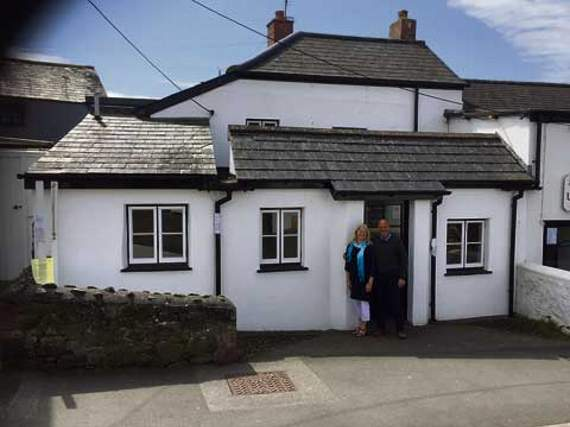
\includegraphics[width=0.75\linewidth]{barrel} The Barrel at Bude is one
of the oldest buildings in Bude and was originally a sea canal worker's
house. It was only the second micropub to open in Cornwall.

\begin{Shaded}
\begin{Highlighting}[]
\NormalTok{barrel <-}\StringTok{ }\KeywordTok{geocode}\NormalTok{(}\StringTok{"36 Lansdown Rd, Bude EX23 8BN, UK"}\NormalTok{)}
\end{Highlighting}
\end{Shaded}

\begin{verbatim}
## Information from URL : http://maps.googleapis.com/maps/api/geocode/json?address=36%20Lansdown%20Rd,%20Bude%20EX23%208BN,%20UK&sensor=false
\end{verbatim}

\hypertarget{the-route}{%
\subsection{The route:}\label{the-route}}

\begin{Shaded}
\begin{Highlighting}[]
\NormalTok{from <-}\StringTok{ "Bude North Cornwall Cricket Club"}
\NormalTok{to <-}\StringTok{ "36 Lansdown Rd, Bude EX23 8BN, UK"}
\NormalTok{route_df <-}\StringTok{ }\KeywordTok{route}\NormalTok{(from, to, }\DataTypeTok{structure =} \StringTok{"route"}\NormalTok{)}
\end{Highlighting}
\end{Shaded}

\begin{verbatim}
## Information from URL : http://maps.googleapis.com/maps/api/directions/json?origin=Bude+North+Cornwall+Cricket+Club&destination=36+Lansdown+Rd,+Bude+EX23+8BN,+UK&mode=driving&units=metric&alternatives=false&sensor=false
\end{verbatim}

\begin{Shaded}
\begin{Highlighting}[]
\KeywordTok{ggmap}\NormalTok{(Bude_roadmap) }\OperatorTok{+}
\StringTok{  }\KeywordTok{geom_point}\NormalTok{(}\DataTypeTok{mapping =} \KeywordTok{aes}\NormalTok{(}\DataTypeTok{x =}\NormalTok{ cricket_grounds_coord}\OperatorTok{$}\NormalTok{lon, }\DataTypeTok{y =}\NormalTok{ cricket_grounds_coord}\OperatorTok{$}\NormalTok{lat)) }\OperatorTok{+}
\StringTok{  }\KeywordTok{geom_label}\NormalTok{(}\DataTypeTok{x =}\NormalTok{ cricket_grounds_coord}\OperatorTok{$}\NormalTok{lon, }\DataTypeTok{y =}\NormalTok{ cricket_grounds_coord}\OperatorTok{$}\NormalTok{lat, }\DataTypeTok{label =} \StringTok{"Cricket Grounds"}\NormalTok{, }\DataTypeTok{hjust =} \DecValTok{1}\NormalTok{, }\DataTypeTok{vjust =} \DecValTok{1}\NormalTok{) }\OperatorTok{+}
\StringTok{  }\KeywordTok{geom_point}\NormalTok{(}\DataTypeTok{mapping =} \KeywordTok{aes}\NormalTok{(}\DataTypeTok{x =}\NormalTok{ barrel}\OperatorTok{$}\NormalTok{lon, }\DataTypeTok{y =}\NormalTok{ barrel}\OperatorTok{$}\NormalTok{lat)) }\OperatorTok{+}
\StringTok{  }\KeywordTok{geom_label}\NormalTok{(}\DataTypeTok{x =}\NormalTok{ barrel}\OperatorTok{$}\NormalTok{lon, }\DataTypeTok{y =}\NormalTok{ barrel}\OperatorTok{$}\NormalTok{lat, }\DataTypeTok{label =} \StringTok{"The Barrel at Bude"}\NormalTok{, }\DataTypeTok{hjust =} \DecValTok{1}\NormalTok{, }\DataTypeTok{vjust =} \DecValTok{1}\NormalTok{) }\OperatorTok{+}\StringTok{  }
\StringTok{  }\KeywordTok{geom_path}\NormalTok{(}\KeywordTok{aes}\NormalTok{(}\DataTypeTok{x =}\NormalTok{ lon, }\DataTypeTok{y =}\NormalTok{ lat), }\DataTypeTok{colour =} \StringTok{"red"}\NormalTok{, }\DataTypeTok{size =} \FloatTok{1.5}\NormalTok{,}
            \DataTypeTok{data =}\NormalTok{ route_df, }\DataTypeTok{lineend =} \StringTok{"round"}\NormalTok{)}
\end{Highlighting}
\end{Shaded}

\includegraphics{Bude_files/figure-latex/unnamed-chunk-22-1.pdf}

\begin{Shaded}
\begin{Highlighting}[]
\KeywordTok{ggmap}\NormalTok{(Bude_watercolor) }\OperatorTok{+}
\StringTok{  }\KeywordTok{geom_point}\NormalTok{(}\DataTypeTok{mapping =} \KeywordTok{aes}\NormalTok{(}\DataTypeTok{x =}\NormalTok{ cricket_grounds_coord}\OperatorTok{$}\NormalTok{lon, }\DataTypeTok{y =}\NormalTok{ cricket_grounds_coord}\OperatorTok{$}\NormalTok{lat)) }\OperatorTok{+}
\StringTok{  }\KeywordTok{geom_label}\NormalTok{(}\DataTypeTok{x =}\NormalTok{ cricket_grounds_coord}\OperatorTok{$}\NormalTok{lon, }\DataTypeTok{y =}\NormalTok{ cricket_grounds_coord}\OperatorTok{$}\NormalTok{lat, }\DataTypeTok{label =} \StringTok{"Cricket Grounds"}\NormalTok{, }\DataTypeTok{hjust =} \DecValTok{1}\NormalTok{, }\DataTypeTok{vjust =} \DecValTok{1}\NormalTok{) }\OperatorTok{+}
\StringTok{  }\KeywordTok{geom_point}\NormalTok{(}\DataTypeTok{mapping =} \KeywordTok{aes}\NormalTok{(}\DataTypeTok{x =}\NormalTok{ barrel}\OperatorTok{$}\NormalTok{lon, }\DataTypeTok{y =}\NormalTok{ barrel}\OperatorTok{$}\NormalTok{lat)) }\OperatorTok{+}
\StringTok{  }\KeywordTok{geom_label}\NormalTok{(}\DataTypeTok{x =}\NormalTok{ barrel}\OperatorTok{$}\NormalTok{lon, }\DataTypeTok{y =}\NormalTok{ barrel}\OperatorTok{$}\NormalTok{lat, }\DataTypeTok{label =} \StringTok{"The Barrel at Bude"}\NormalTok{, }\DataTypeTok{hjust =} \DecValTok{1}\NormalTok{, }\DataTypeTok{vjust =} \DecValTok{1}\NormalTok{) }\OperatorTok{+}\StringTok{  }
\StringTok{  }\KeywordTok{geom_path}\NormalTok{(}\KeywordTok{aes}\NormalTok{(}\DataTypeTok{x =}\NormalTok{ lon, }\DataTypeTok{y =}\NormalTok{ lat), }\DataTypeTok{colour =} \StringTok{"red"}\NormalTok{, }\DataTypeTok{size =} \FloatTok{1.5}\NormalTok{,}
            \DataTypeTok{data =}\NormalTok{ route_df, }\DataTypeTok{lineend =} \StringTok{"round"}\NormalTok{)}
\end{Highlighting}
\end{Shaded}

\includegraphics{Bude_files/figure-latex/unnamed-chunk-23-1.pdf}


\end{document}
